\section{Simulation Analysis}
\label{sec:simulation}


%Introduzir a cena do ngspice costume
%Mostrar a cena optimizada e explicar o porque de termos usado estes valores diferentes

\indent
 
This section discusses the circuit simulation, performed using {\it Ngspice}. 

This circuit was entered into the {\it Ngspice} simulation environment. This tool is used to simulate analog electronic circuits and predict circuit behaviour. 

After having the base circuit description, the parameters have been chosen by trial and error. The final values are present on the following table (table \ref{tab:InputParam}):

\begin{table}[H]
  \centering
  \begin{tabular}{|l|r|}
    \hline    
    {\bf Name} & {\bf Value} \\ \hline
    \input{../Analysis/inputs.tex}
  \end{tabular}
  \caption{Input Parameters}
  \label{tab:InputParam}
\end{table}


In this iterative progress, we arrived at these conclusions about each main parameter:
 

\begin{itemize}
    \item\textbf{C1 and R1}
    These components have a big impact on the central frequency. When increased the central frequency is reduced substantially, mostly due to the fact that it lowers the high cut-off frequency and therefore widens the frequency bandwidth. The gain, however, reacts in the opposite way, increasing with them.
    %este está bom
    \item\textbf{R3 and R4}
    These resistors are responsible for the gain and, as stated before, R3 needs to be 99 times bigger than R4, in order to achieve the desired gain. Furthermore, these do not have a meaningful effect on the central frequency.
    \item\textbf{C2 and R2}
     These components have both an impact on the gain and on the central frequency. When the resistance or the capacitance is increased, both the gain and the central frequency go down. 
     
\end{itemize}    

 
\subsection{OP Analysis}

\indent

With the parameters honed in, the OP analysis was performed, visible on table \ref{tab:OP_ngs}:

\begin{table}[H]
  \centering
  \begin{tabular}{|l|r|}
    \hline    
    {\bf Name} & {\bf Value} \\ \hline
    @c[i] & 0.000000e+00\\ \hline
@gcs[i] & -2.04136e-04\\ \hline
@r1[i] & 1.945229e-04\\ \hline
@r2[i] & -2.04136e-04\\ \hline
@r3[i] & -9.61363e-06\\ \hline
@r4[i] & 1.156284e-03\\ \hline
@r5[i] & 2.041365e-04\\ \hline
@r6[i] & 9.617613e-04\\ \hline
@r7[i] & 9.617613e-04\\ \hline
v(1) & 5.008942e+00\\ \hline
v(2) & 4.808960e+00\\ \hline
v(3) & 4.394159e+00\\ \hline
v(4) & 0.000000e+00\\ \hline
v(5) & 4.837862e+00\\ \hline
v(6) & 5.474755e+00\\ \hline
v(7) & -2.00872e+00\\ \hline
v(8) & -2.97092e+00\\ \hline

  \end{tabular}
  \caption{OP Analysis}
  \label{tab:OP_ngs}
\end{table}

\subsection{Frequency Analysis}

\indent

After the OP analysis, it is possible to create a frequency analysis, that can be seen on the next 2 graphs (Figure \ref{fig:FreqANGS}):

\begin{figure}[H]
\centering
\begin{subfigure}{.49\textwidth}
  \centering
  \includegraphics[width=.8\linewidth, trim={2cm 1.5cm 0.5cm 6cm}, clip]{../Simulation/vo1f_m.pdf}
  \caption{Magnitude}
\end{subfigure}%
\begin{subfigure}{.49\textwidth}
  \centering
  \includegraphics[width=.8\linewidth, trim={2cm 1.5cm 0.5cm 6cm}, clip]{../Simulation/vo1f_ph.pdf}
  \caption{Phase}
\end{subfigure}
\caption{Frequency analysis}
\label{fig:FreqANGS}
\end{figure}


With this done, the final parameter for the band pass filter can be obtained as well as the impedances of the circuit:

\begin{table}[H]
  \centering
  \begin{tabular}{|l|r|}
    \hline    
    {\bf Name} & {\bf Value} \\ \hline
    \input{../Simulation/freq_tab.tex} %cHANGE THIS
  \end{tabular}
  \caption{Output parameters}
  \label{tab: OutputParamNGS}
\end{table}


\begin{table}[H]
  \centering
  \begin{tabular}{|l|r|}
    \hline    
    {\bf Name} & {\bf Value} \\ \hline
    \input{../Simulation/Zin_tab.tex}
    \input{../Simulation/Zout_tab.tex}
  \end{tabular}
  \caption{Input and output impedances}
  \label{tab: ImpNGS}
\end{table}

Finally, using an arbitrary frequency, we can perform a transient analysis:


\begin{figure}[h!]
    \centering
  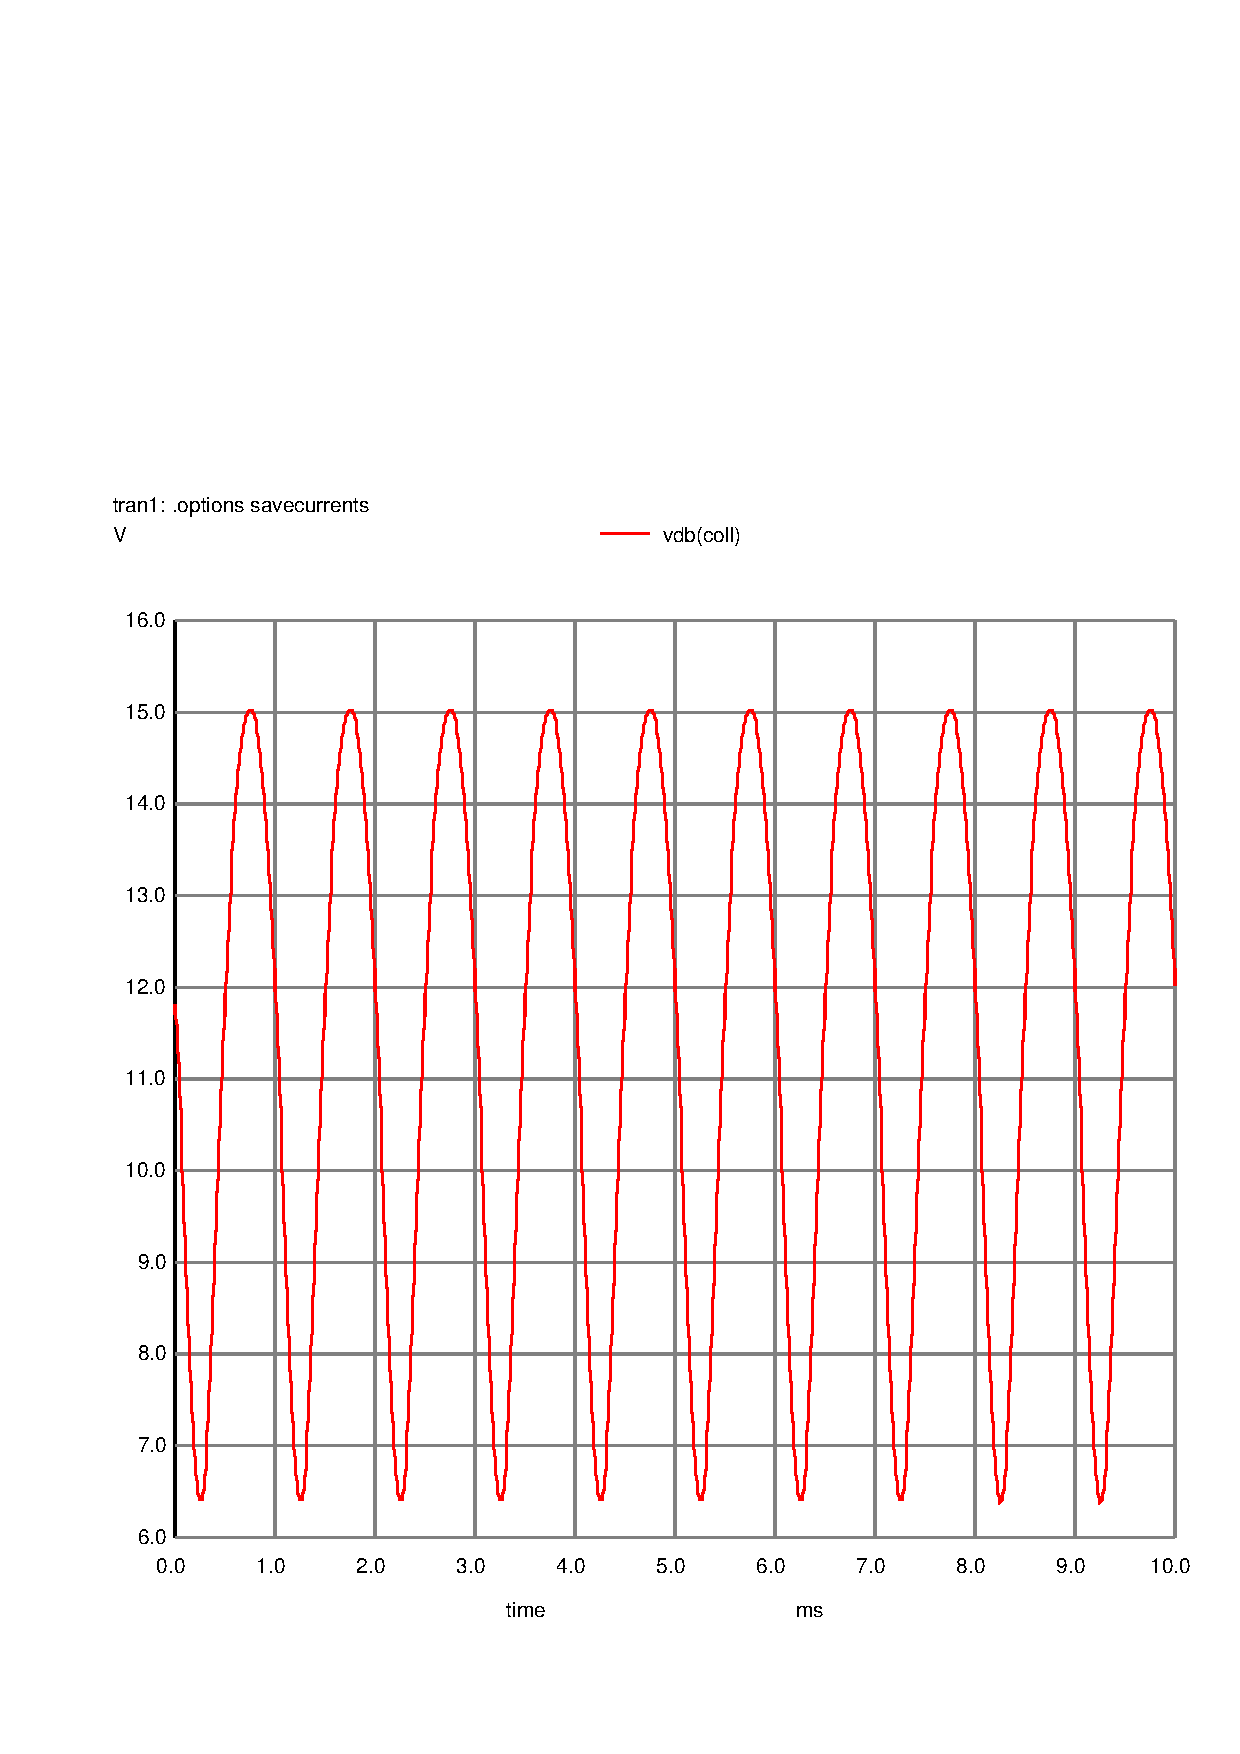
\includegraphics[width=.6\linewidth, trim={2cm 1.5cm 0.5cm 6cm}, clip]{../Simulation/vo1.pdf}
  \caption{Transient analysis - Voltage output}
  \label{tab:TransNGS}
\end{figure}


As shown, the signal is greatly amplified and shows no visible distortions, since we used a frequency which was not dampened by the system
